\appendix 

\chapter{Resources}

\section{Hardware Architecture Overview}
\label{sec:hw_arch}

\begin{figure}[H]
\centering
%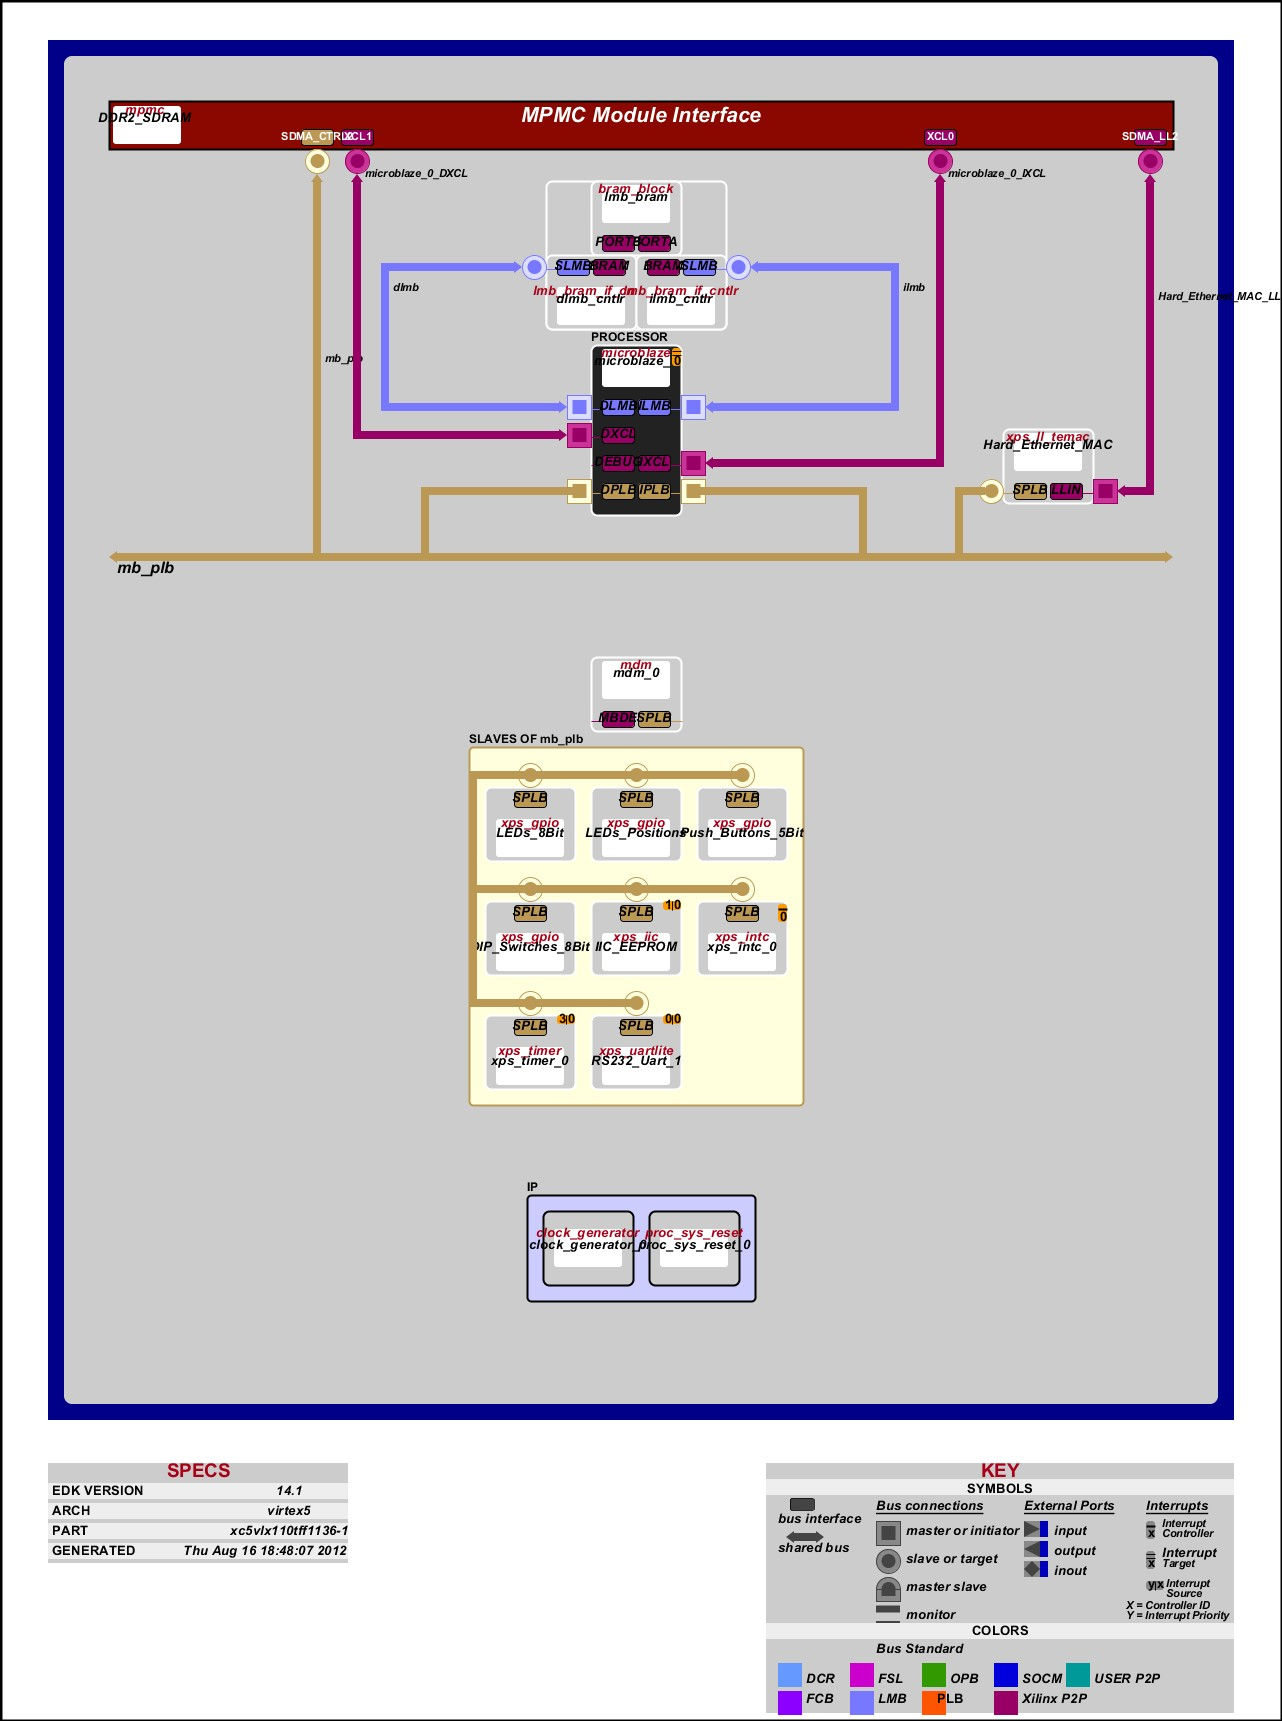
\includegraphics[width=0.9\textwidth]{system_blkd.jpg}
\end{figure}


\section{Hardware Project Configurations}

The configuration files contain more than 800 lines, being too much to include them directly in the project report. Therefore the \textit{Microprocessor Hardware Specification (mhs)} and \textit{User Constraint File (ucf)} files can be downloaded as part of the projects for \textit{\gls{xps}} and the \textit{Xilinx ISE Project Navigator} from the following address: \url{http://www.peschuster.de/ies-project/IesHttpProject-Hardware.zip}.
\\

\section{Linux Kernel Assets}

\subsection{Configuration}

The Linux kernel configuration file contains more than 1,200 lines and is therefore not included directly within this appendix, but can be downloaded together with all other scripts concerning the software part of this project from the following address: \url{http://www.peschuster.de/ies-project/IesHttpProject-Software.zip}.

Here are the configuration settings specific for the \textit{MicroBlaze} processor used in this project:

\begin{verbatim}
CONFIG_KERNEL_BASE_ADDR=0x50000000
CONFIG_XILINX_MICROBLAZE0_FAMILY="virtex5"
CONFIG_XILINX_MICROBLAZE0_USE_MSR_INSTR=1
CONFIG_XILINX_MICROBLAZE0_USE_PCMP_INSTR=1
CONFIG_XILINX_MICROBLAZE0_USE_BARREL=1
CONFIG_XILINX_MICROBLAZE0_USE_DIV=1
CONFIG_XILINX_MICROBLAZE0_USE_HW_MUL=2
CONFIG_XILINX_MICROBLAZE0_USE_FPU=0
CONFIG_XILINX_MICROBLAZE0_HW_VER="8.30.a"
\end{verbatim}

 

\subsection{Patches}
\label{subsec:pvr_patch}

Path for correct recognition of the latest \textit{MicroBlaze} processor versions with enabled \gls{pvr}:

\begin{verbatim}
commit 9be0160c855d1740f392d74a90197421c1380946
Author: Peter Schuster <schuster.pe@gmail.com>
Date:   Sat Sep 8 19:48:56 2012 +0200

    Added new MicroBlaze versions.

diff --git a/arch/microblaze/kernel/cpu/cpuinfo.c b/arch/microblaze/kernel/cpu/cpuinfo.c
index 54194b2..783c7087 100644
--- a/arch/microblaze/kernel/cpu/cpuinfo.c
+++ b/arch/microblaze/kernel/cpu/cpuinfo.c
@@ -35,6 +35,8 @@ const struct cpu_ver_key cpu_ver_lookup[] = {
 	{"8.00.b", 0x13},
 	{"8.10.a", 0x14},
 	{"8.20.a", 0x15},
+        {"8.20.b", 0x16},
+        {"8.30.a", 0x17},
 	{NULL, 0},
 };
\end{verbatim}

The patch file "\texttt{new-microblaze-versions.patch}" is also included in the zip archive available at \url{http://www.peschuster.de/ies-project/IesHttpProject-Software.zip}.
\\

\subsection{syslog.tcl}
\label{subsec:syslog}

\begin{verbatim}
proc mb_mrd_w { address } {
    return 0x[ string range [mrd $address 1 w] 12  19]
}

proc syslog { } {
    set bufaddr 0xc04d3c30
    set bufsize 0x00020000

    set startaddr $bufaddr
    set endaddr [expr $bufaddr + $bufsize]
	
    set fp [open "syslog_1.txt" w]

    puts $fp "Displaying Linux syslog buffer of $bufsize length at $bufaddr"
	
    while {$startaddr < $endaddr} {
        # Read 4 bytes of text
        set mval [ mb_mrd_w $startaddr ]

        # Display the word of text, a byte at a time
        set shift 24
        while {$shift >= 0} {
            set char [expr [expr $mval >> $shift] & 0xff]
            # NULL ? End of string.
            if {$char == 0} {
                return
            }
            set char [format "%c" $char]
            puts -nonewline $fp "$char"

            incr shift -8
        }

        incr startaddr 4
    }
    puts $fp ""
    close $fp
}
\end{verbatim}

The file "\texttt{syslog.tcl}" is also included in the zip archive available at \url{http://www.peschuster.de/ies-project/IesHttpProject-Software.zip}.
\\

\subsection{pack-fs.sh}
\label{subsec:pack-fs}

\begin{verbatim}
#!/bin/bash

f=`dirname "$0"`

cd "$f/complete"
find . -print | cpio -H newc -o | gzip > "../complete_fs.cpio.gz"
\end{verbatim}

The file "\texttt{pack-fs.sh}" is also included in the zip archive available at \url{http://www.peschuster.de/ies-project/IesHttpProject-Software.zip}.
\\

\subsection{Device Tree Generator and Source}
\label{subsec:dts-generator}

The latest version of the \textit{Device Tree Generator} \gls{bsp} can be downloaded from the site of Michal Simek (\url{http://www.monstr.eu/wiki/lib/exe/fetch.php?media=fdt:fdt:logs:device-tree_latest.tar.gz}.

It is also available in version 1.3 from the url \url{http://www.peschuster.de/ies-project/device-tree-1-3.zip}, as used in this project.

The dts file (\texttt{xupv5.dts}) for the hardware system used in this project is part of the zip archive available at \url{http://www.peschuster.de/ies-project/IesHttpProject-Software.zip}.
\\

\section{Image files}

The \textit{bitstream} (\texttt{system.bit}) and Linux kernel image (\texttt{simpleImage.xupv5}) files for the \textit{Xilinx XUPV5-LX110T} board and described hardware system are available for download at \url{http://www.peschuster.de/ies-project/IesHttpProject-Images.zip}.


\section{SoC Environment Evaluation Program}
\label{sec:nginx-env-eval}

\textbf{C program}
\begin{verbatim}
#include <stdio.h>
#include <stdlib.h>
#include <signal.h>
#include "xparameters.h"
#include "xil_cache.h"

void print(char *str);

int main()
{
    #ifdef XPAR_MICROBLAZE_USE_ICACHE
        Xil_ICacheEnable();
    #endif
    #ifdef XPAR_MICROBLAZE_USE_DCACHE
        Xil_DCacheEnable();
    #endif

    print("Env analysis (size_of): \r\n \r\n");

    printf("size of int: %d \r\n", (int)sizeof(int));
    printf("size of long: %d \r\n", (int)sizeof(long));
    printf("size of long long: %d \r\n", (int)sizeof(long long));
    printf("size of void *: %d \r\n", (int)sizeof(void *));
    printf("size of sig_atomic_t: %d \r\n", (int)sizeof(sig_atomic_t));
    printf("size of size_t: %d \r\n", (int)sizeof(size_t));
    printf("size of off_t: %d \r\n", (int)sizeof(off_t));
    printf("size of time_t: %d \r\n", (int)sizeof(time_t));

    Xil_DCacheDisable();
    Xil_ICacheDisable();

    return 0;
}
\end{verbatim}

\textbf{Result}
\begin{verbatim}
size of int: 4
size of long: 4
size of long long: 8
size of void *: 4
size of sig_atomic_t: 4
size of size_t: 4
size of off_t: 4
size of time_t: 4
\end{verbatim}